\documentclass[a4paper, usenatbib, 12pt]{article}
\usepackage{subfig}
\usepackage{float}
\usepackage{wrapfig}
\usepackage{graphicx}
\usepackage{amsmath}
\usepackage{amssymb}
\usepackage{booktabs}
\usepackage{cite}
\usepackage[icelandic,spanish,english]{babel}
\usepackage[T1]{fontenc}
\usepackage[utf8]{inputenc}
\usepackage[top=3.5cm, bottom=2.5cm, left=3.5cm,right=3.5cm]{geometry} 

%----------------------New commands -------------------

\newcommand{\tol}{Tololo 1214-277}
\newcommand{\lya}{Ly$\alpha$}
\newcommand{\hb}{H$\beta$}
\newcommand{\ha}{H$\alpha$}
\newcommand{\oiii}{[OIII]}
\newcommand{\oii}{[OII]}
\newcommand{\nii}{[NII]}
\newcommand{\esca}{erg cm$^{-2}$ s$^{-1}$ \AA$^{-1}$}
\newcommand{\esc}{erg cm$^{-2}$ s$^{-1}$}
\newcommand{\es}{erg s$^{-1}$}
\newcommand{\esa}{erg s$^{-1}$}
\newcommand{\kms}{km s$^{-1}$}
\newcommand{\apj}{ApJ}  
\newcommand{\jcap}{JCAP}  
\newcommand{\apjs}{ApJS}  
\newcommand{\apjl}{ApJL}  
\newcommand{\aj}{AJ}  
\newcommand{\mnras}{MNRAS}  
\newcommand{\mnrassub}{MNRAS accepted}  
\newcommand{\aap}{A\&A}  
\newcommand{\aaps}{A\&AS}  
\newcommand{\araa}{ARA\&A}  
\newcommand{\nat}{Nature}  
\newcommand{\physrep}{PhR}
\newcommand{\pasp}{PASP}    
\newcommand{\pasj}{PASJ}    
\def\simgt{\lower.5ex\hbox{\gtsima}}
\def\simlt{\lower.5ex\hbox{\ltsima}}
%------------------------------------------------------

\begin{document}
\pagestyle{empty}
\noindent
\textbf{Þú ert jörðin}
\\
\\
JEFR$^{1}$, MCRG$^1$, JNGC$^2$, MD$^3$
\\
\\
\scriptsize
{$^1$ Bogota
\\
$^2$ Tucson
\\
$^3$ Oslo
\normalsize
\\
\\
\textbf{
Star-forming Compact Dwarf Galaxies (CDGs) resemble the expected pristine conditions of the first galaxies.  
Until these early galaxy generations are observationally
detected, CDGs are the best systems to test our ideas on primordial
galaxy formation and evolution.  
Here we report on one of such CDGs, \tol, which presents
features in its Lyman-$\alpha$ emission thad had evaded theoretical
interpretation so far. 
We show that these special features, a symmetric triple peaked
emission line, are naturally explained by gas rotation.  
We find that the Lyman-$\alpha$ emission region in \tol\ should
have a rotational velocity of $V_{r}=300$ km s$^{-1}$ and a neutral
Hydrogen column density of $\log N_{HI} / \mathrm{atoms\ cm}^{-2} =
  20.5$.   
Using archival observational information we find that
the diameter for that region should be in the range of
$110$ pc $<D<$ $340$ pc and its total dynamical mass 
should be between $2.1\times 10^{9}$M$_{\odot}$ $<M_D<$  $6.6\times
10^{9}$M$_{\odot}$. 
This dynamical mass is at least $16\pm 9$ times
larger than the neutral mass hydrogen.
We argue that a possibility to explain the excess in
dynamical mass is the presence of a super-massive black hole. }



%\section{Introduction}

1. [General paragraph about the first galaxies and CDGs]


2. [General paragrph about the expected Lyman-alpha emission,
  LARS]. Almost fifty years ago \cite{PartridgePeebles} it was
realized that young galaxies could be detected through a stron
Lyman-$\alpha$ line emission.  This theoretical prediction was only
confirmed XX year later. 
Currently, Lyman Alpha Emitting galaxies are commonly measure in
surveys. 
The presence of this line provides confirmation of the distance of a
galaxy and also provides clues about the stellar population powering
the emission.

Lyman alpha emission is not exclusive of high redshift galaxies. It
does, require a low dust content to avoid complete extinction and an
source of ionizing radiation.  This has motivated the creation of
local Universe surveys to perform a detailed study of the Lyman-alpha
emission \cite{LARS}. A nearby simple permits the study of other
indicators that might be more difficult to obtain for distant galaxies
such as morphology, dust attenuation, neutral hydrogen contents and
ionization state. 


3. [Observations require interpretation, common features and
  models]. The Lyman-$\alpha$ line is resonant. A yman-$\alpha$ photon
will follow a difussion-like process before escaping the galaxy or
being absorbed by dust. This makes it hard to interpret Lyman-alpha
line observations as the reulting profile is sensitive to the
dynamical, chemical and thermal conditions in the interstellar
medium. State-of-the-art models use mon.

4. [Rotation and the expected features.]
It has been shown that rotation also imprints an effect on the
Lyman-alpha morphology. 
The most important consequence of rotation is that spherical 
symmetry is broken.
The line morphology now depends on the viewing angle respect to the
rotation axis.  
For a line of sight perpendicular to the rotation axis the intensity
and the line center and the line width increase with rotational
velocity.  
When the rotational velocity is close to the half-line width of the
static line, the line becomes single peaked as it is observed in
\tol, a unique feature that other theoretical models find
impossible to reproduce.
 

5. [The charachteristics of the dwarf galaxy of interest as a puzzling
system]

\tol was first observed by ... it is a compact 
dwarf galaxy and does not have old stars. 

The Ly$\alpha$ emission line was first observed in the \tol
galaxy by \cite{Thuan97}. It has two main important features which 
make this a very uncommun LAE. First it shown a symmetric profile 
which is , Second the Ly$\alpha$ line is not shifted with respect to 
the H$\beta$ line.  Blue compact Dwarf Galaxy


6. [The results of the fit + Physical picture using other results]

Figure 1. shows the observational data for \tol

with the overplot from
our best fit model from the full radiative transfer simulation. 
The parameters for the best fit are
$v_{max}=300$\kms, $\tau=1\times10^7$, $T=1.5\times 10^{4}$K and a
viewing angle $\theta<30$ degrees. 



\begin{figure}
\begin{center}
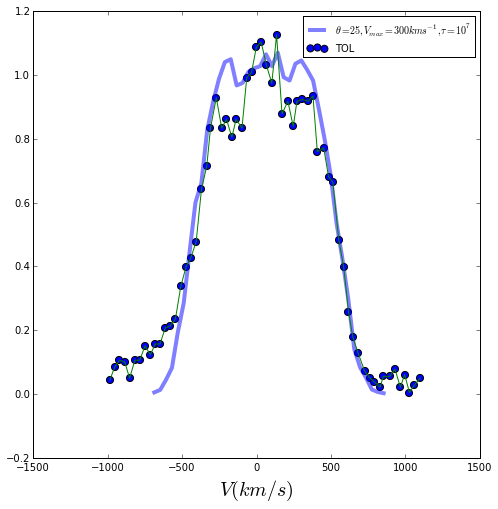
\includegraphics[width=0.8\textwidth]{tolfit.png}
\caption{Nice fit}
\end{center}
\end{figure}



%6. Comparison of these results against other observational 
Assuming spherical symmetry and a homogeneous gas distribution we
estimate the total neutral hydrogen mass to be on the order of
$M\approx m_H\tau^3\sigma^{-3}n^{-2}$, where $m_H$ is the mass a
Hydrogen's atom, $\tau$  the optical depth, $\sigma$ is the cross
section at the line's center and $n$ is the number density of neutral
Hydrogen atoms. 
For this system we estimate that for average values of $n=1\times
10^3$ the total hydrogen mass is $M\times 10^{14}$M$_{\odot}$. 
However, blind HI
surveys have put an upper limit in the neutral hydrogen mass of ???

7. [Possible interpretation of this results]

8. [Implications for outflow+rotation in existing samples.] Why are
not more examples of triple peaked emission? 
The ubiuquity of galaxy outflows overimposed to the rotation
transforms the line into the common double or single peaked
observations.  


9. [Future outlook]


\bibliography{references}{}
\bibliographystyle{plain}

\newpage 

\section*{\tol\ characteristics}


\begin{table}
\begin{center}
\begin{tabular}{lc}
$\alpha$(2000)$^{a}$ & 12h17min17.1s\\
$\delta$(2000)$^{b}$ & -28d02m32s\\
$l$, $b$ (deg) & 294, 34\\
$m_V$ & 17.5\\
$v$(km s$^{-1}$) & 7795
\end{tabular}
\end{center}

\caption{Observational characteristics of TOL1214-277
  \cite{Thuan97}\\} 
\end{table}

\tol receeding velocity is $7785\pm 50$km s$^{-1}$, which translates
into a distance of $106.6$ Mpc (Hubble constant 73 Mpc km$^{-1}$
s$^{1}$)
Its metallicity is $\sim Z_{\odot}/24$ \cite{Izotov04} as derived from optical
spectroscopy. 

The observed flux for the Lyman alpha line is $\sim
8.1\times 10^{-14}$ erg cm$^{-2}$ s$^{-1}$ \cite{Thuan97}
and a Equivalent Width of $70$\AA and its H$\beta$ flux is 
$1.62\times 10^{-14}$ erg cm$^{-2}$ s$^{-1}$ cm${-2}$
\cite{Izotov04} which gives a Ly$\alpha$/H$\beta$ flux ratio of
4.9$\pm$0.1. 
Comparing this ratio with the theoretical expectation from case B
recombination of $23.3$ \cite{Hummer1987} one can estimate an escape
fraction of $20$\% for Ly$\alpha$ radiation.

The optical emission  comes from a   region with approximate diameter
?? \cite{Fricke01}. 

\section*{MCMC constraints}

\section*{Physical Interpretation}

Interpretation by \cite{mashesse03}.

There is an upper limit for the  
integrated flux of $<0.10$ Jy km s$^{-1}$, which translates into a
upper limit for the HI mass of $M<2.65\times 10^{8}$ M$_{\odot}$
\cite{pustilnikmartin07}. 
From the optical depth of $10^7$ and the non-detection in the HI line,
we have an upper limit for the size where the Lya emission comes of
$D<0.34$kpc. 

 For an homogeneous sphere the HI optical depth from its can be
 written as $\tau = \sigma_0 n D/2$, where $\sigma_0=5.898\times
10^{-14}$cm$^{-2}$ is the Lyman$\alpha$  optical depth at the 
line's center, $n$ is the number density and $D$ is the sphere's
diameter. 
From this we can impose additional constrains on $D$ from the tipical
values of the Hydrogen number density and our constrain on
$\tau=10^{7}$.  Using a range of $1<n/\mathrm{atoms/cm}^{-3} <
10^{-3}$. This gives us a range of $0.11 < D/\mathrm{kpc}<100$. 
Together from the total HI mass we have thus that the HI region should
have a diameter of $0.11 < D/\mathrm{kpc}<0.34$.



This can be rewritten in terms of the gas' temperature $T$ and column
density $N_{H}$as $\tau = 3.31 \times 10^{-14} (10^{4}\mathrm{K}/T)^{1/2}
(N_{H}/\mathrm{atoms\ cm}^{-2})$.  

This allows us to approximate the total hydrogen mass as
\begin{equation}
M_{H} = m_{H}  N_{H} D^{2} = 226\times \tau  \left(\frac{T}{10^4
  \mathrm{K}}\right)^{1/2}\left(\frac{D}{\mathrm{kpc}}\right)^2M_{\odot}
\end{equation}





On the other hand, we have an estimate for the dynamical mass from the
galaxy size $D$ and its rotational velocity $V$:



\begin{equation}
M_{T} = \frac{V^{2}D}{G} = 2.16\times10^{5}
\left(\frac{V}{\mathrm{km\ s}^{-1}}\right)^2\left(\frac{D}{\mathrm{kpc}}\right) M_{\odot}
\end{equation}


From this limit and the rotational velocity of $300$ km/s and the
limit in the size $D$ we have limits of for the dynamical mass of
$2.1\times 10^{9}$M$_{\odot}$ $<M_D<$  $6.6\times 10^{9}$M$_{\odot}$.

which is at least $7$ to $25$ times larger than the H$I$ mass. 


\section*{Joint Effect of Rotation and Outflow}

The almost complete absence of outflows is a central requirement for
reproducing the lyman alpha line in \tol. In this section we present
some results on the exploration of the presence of outflows join with
the bulk rotation. We defer a detailed exploration of this effects for
another publication. 

Figure XX shows the results of four different models. a) pure rotation
($V_{\rm rot}=100$ km s$^{-1}$), b) pure outflow ($V_{\rm out}=100$ km
s$^{-1}$), c) mixed outflow with rotation ($V_{\rm rot}=100$ km s$^{-1}$)($V_{\rm rot}=25$ km s$^{-1}$).



\end{document}

%% interpretation

